\section{Konzeption}



\subsection{Vergleich zu bestehender Software}

Im Wesentlichen hat MultiTextCompare zwei zentrale Funktionen. Zum einen den Vergleich beliebig vieler textbasierter Dateien, und zum anderen die Anzeige der \acrshort{diff} für bis zu drei Dateien. Es gibt Anwendungen, die eine prozentuale Ähnlichkeit für zwei Dateien anzeigen können. Jedoch liegt dort der Fokus auf dem semantischen Textvergleich im Sinne der Plagiatserkennung. Wie bereits in \ref{String similarity Algorithmen} erwähnt, arbeitet MultiTextCompare rein zeichenbasiert und reagiert daher nicht auf sprachliche Ähnlichkeiten bei der Ähnlichkeitsbewertung. 

Im Bereich der Diff-Tools existieren häufig Programme, die die Diff für maximal zwei Dateien anzeigen können. Eine Ausnahme ist hierbei die Anwendung \textit{KDiff3}, welche einen Vergleich für drei Dateien zulässt. Um eine Diff für drei Dateien zu erzeugen, muss eine der Dateien als Referenz markiert werden. Für die drei Inputdateien A,B,C mit A als Referenz entstehen dann die Vergleiche $\{A,B\}, \{A,C\}$, während MultiTextCompare keine Datei als Referenz festlegt und jede Datei mit jeder vergleicht. 

Um Unterschiede farbkodiert darzustellen, ist ein Ansatz mit nur zwei Vergleichen zwar für den Benutzer einfacher nachzuvollziehen und zudem performanter als alle drei Vergleiche auszuführen, aber dafür gehen Informationen verloren. Gerade dann, wenn 3 ähnliche Dateien für die Diff ausgewählt werden, kann es interessant sein, die Unterschiede zwischen allen Dateien gleichermaßen zu betrachten.

%Vllt Tabelle mit Farben einfügen%

\subsection{Anforderungen}

Für die Entwicklung der Software MultiTextCompare sind einige funktionale und nicht-funktionale Anforderungen entstanden. Die funktionalen Anforderung wurden bereits größtenteils innerhalb des Einleitungskapitels beschrieben. Zu den nicht-funktionalen Anforderungen gehört der Aspekt, dass die Software speziell für die Laborrechner der Technischen Hochschule Köln entworfen werden soll. Dafür soll Java in der Version 1.7.0\_75 für 32 Bit Systeme verwendet werden. Als IDE soll Eclipse (Release Luna SR2) verwendet werden, um die Code-Basis auch für die Installationen im Labor nahtlos lauffähig zu machen und um nicht auf generierte \acrfull{jar} angewiesen zu sein. Zudem soll die Software primär mit Windows 7 kompatibel sein.

Eine weitere Anforderung ist die einfache Benutzbarkeit. Um dies zu gewährleisten sollen alle notwendigen Funktionen auf den ersten Blick erkennbar, und jegliche Auswahlmöglichkeiten annotiert sein, um dem Benutzer Hilfestellung zu leisten.

\subsection{Architektur}\label{architektur}

Als Architektur wurde auf eine 3-Schichten-Architektur zurückgegriffen. Diese ist grob in Abb. \ref{fig:architektur} als UML-Komponentendiagramm dargestellt. Die Komponenten sind hier als logische Zusammenfassungen von Java Klassen gemeint, wobei jede Komponente aus mindestens einer Java Klasse besteht und genau ein Aufgabengebiet erfüllt. Zusätzlich handelt es sich bei den verwendeten Pfeilen um \textit{<<uses>>} Relationen, wobei die Annotationen zwecks einer besseren Lesbarkeit weggelassen wurden. Aus dem gleichen Grund wurde auf die Darstellung von Interfaces und detailierten Relationen zwischen den Schichten verzichtet.

\begin{figure}[!htb]
    \centering
    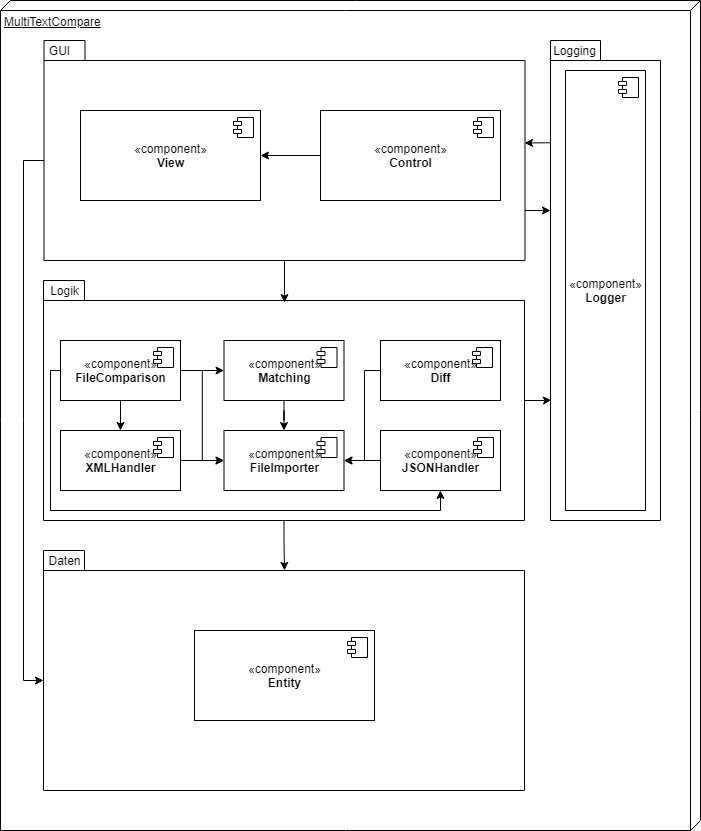
\includegraphics[scale=0.5]{images/Komponenten_MTC_final.png}
    \caption{Übersicht der Architektur}
    \label{fig:architektur}
\end{figure}

In der obersten Schicht liegen alle Java-Klassen, die mit der UI in Verbindung stehen. Dort existiert eine Teilung zwischen Klassen der View-Komponente und denen der Control-Komponente. View-Klassen initialisieren bestimmte UI-Elemente und bestimmen deren Aussehen. Jede View-Klasse, die dynamische Inhalte anzeigen kann, hat eine zugehörige Controller-Klasse für das Event-Handling und Verändern der UI. 

In der Logikschicht befinden sich die Komponenten, die für die Algorithmen und das File-Handling verantwortlich sind. Jede öffentliche Klasse dieser Schicht bietet dabei ein Interface an die GUI-Schicht an. Die Komponente \textit{FileImporter} ist u.\,a. dafür zuständig, die vom Benutzer ausgewählten Dateien zu finden, sie als temporäre Dateien zu klonen und auf die Originaldateien zu mappen. Alle anderen Komponenten greifen auf diese Map zu, um die Dateien weiter zu verarbeiten. Die \emph{FileComparison}-Komponente beherbergt die Vergleichsalgorithmen, die die Werte für die Matrix berechnen. Für Operationen an XML und JSON wie die Filterung oder Sortierung sind die Komponenten XMLHandler bzw. JSONHandler zuständig.

Die Datenschicht ist letztlich eine rein logische Trennung von den anderen Schichten. Da keine Datenbank existiert, gibt es keine Notwendigkeit für CRUD-Komponenten. Die im Diagramm gezeigte Entity-Komponente beherbergt also nur Java Objekte, die für die Speicherung von Daten zur Laufzeit notwendig sind. Dazu gehört bspw. die Klasse \,\textit{IConfigImpl}, die ein Klassenattribut für jede konfigurierbare Einstellung enthält und zur Laufzeit mit dem Inhalt der aktiven Konfigurationsdatei befüllt wird. Jede Entitätsklasse besitzt ebenfalls ein zugehöriges Interface, welches die \emph{Getter} und \emph{Setter} an höhere Schichten übergibt.

Die Logging-Komponente existierte zwar in Version 1.0 noch nicht, da sie aber die einzige architektonische Änderung während der Bearbeitung dieser Arbeit ist, wird sie hier bereits aufgeführt. Sowohl Komponenten aus der Logik-Schicht als auch aus der GUI-Schicht, können Fehler loggen. Diese Fehler werden in der UI dargestellt, falls das entsprechende Log-Level vom Benutzer gesetzt ist. Die genauere Funktionsweise wird in Kapitel \ref{logging} beschrieben. Informationen zu den einzelnen Klassen, Interfaces und Methoden können als Javadoc direkt über MultiTextCompare im Browser geöffnet werden.


